There are two possible cases that results in an energy imbalance in the
detector, the first one occurs in beyond Standard Model physics, that often
involves the presence of particles that interact weakly or not at all with
normal matter. These particles are not detected thus leaving an energy imbalance
in the detector. In the second case, the decay products in the final state do
not have enough energy to be detected. To better understand this second category
of events, consider \cref{fig:susy_standard} that shows the decay topology of
squark pair production with a neutralino and two jets in the final state. Using
the two body decay energy and momentum relations (see~\cite{PDG}):
\begin{equation}
  \label{eq:93}
  E_q = \frac{M_{\, \tilde{q}}^2 - m_{\, \tilde{\chi}_{\, 1}^{\, 0}}^2 + m_q^2}{2
    M_{\, \tilde{q}}},
\end{equation}
\begin{equation}
  \label{eq:94}
  |\vec{p}_q| = |\vec{p}_{\, \tilde{\chi}_{\, 1}^{\, 0}}| = \frac{\left[ \left(
        M_{\, \tilde{q}}^2 - (m_q + m_{\, \tilde{\chi}_{\, 1}^{\, 0}})^2
      \right) \left( M_{\, \tilde{q}}^2 - (m_q - m_{\, \tilde{\chi}_{\, 1}^{\,
            0}})^2 \right) \right]^{1/2}}{2 M_{\, \tilde{q}}}
\end{equation}
where $M_{\, \tilde{q}}$ is the squark center of mass energy,
$m_{\, \tilde{\chi}_{\, 1}^{\, 0}}$ is the neutralino mass and $m_q$ is the
quark mass. Neglecting the quark mass ($m_q = 0$) we get that:
\begin{equation}
  \label{eq:95}
  E_q = \frac{M_{\, \tilde{q}}^2 - m_{\, \tilde{\chi}_{\, 1}^{\, 0}}^2}{2 M_{\,
      \tilde{q}}},
\end{equation}
\begin{equation}
  \label{eq:96}
  |\vec{p}_q| = |\vec{p}_{\, \tilde{\chi}_{\, 1}^{\, 0}}| = \frac{M_{\,
      \tilde{q}}^2 - m_{\, \tilde{\chi}_{\, 1}^{\, 0}}^2}{2 M_{\, \tilde{q}}}.
\end{equation}
The quark will hadronize in the calorimeter and if it has enough energy can be
reconstructed as jet. On the other hand, if the energy of the quark is below a
given threshold it is not detected and thus results in missing energy.

It can be seen from \cref{eq:95,eq:96} that when the mass of the neutralino
approaches the mass of the quark this results in a low energy jet that might
escape detection. Thus if the mass difference between the particles is small,
the sensitivity to new physics signal of many standard SUSY searches is reduced
due to the low amount of missing energy and the low transverse momentum of the
associated jets. If the event has an initial state radiation, as depicted in
\cref{fig:susy_compressed}, the amount of missing energy and the corresponding
transverse momentum jets will be large leading thus to a clean signature for the
monojet.

Events with an energetic jet $\pt$ and large $\met$ in the final state thus
constitute a clean signature for new physics searches at hadron
colliders. Signals that can be studied with this experimental signature include
the production of WIMPS, the ADD model for large extra dimensions and SUSY\@.

Supersymmetry is expected to solve some of the shortcomings of the Standard
Model mentioned in \cref{sec:open-quest-stand}, it is possible to estimate, from
\cref{eq:delta_mh}, the scale at which new physics is expected. Using m$_H$ =
125~GeV~\cite{PDG}, we get that $\Lambda \approx 1$~TeV. If the naturalness
criterion holds, we expect the two main experiments at LHC, ATLAS and CMS, to
find signal for new physics at the TeV scale.

\begin{figure}[!h]
  \centering
  \begin{subfigure}[t]{.48\linewidth}
    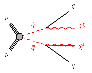
\includegraphics[width=\linewidth]{susy_standard}
    \caption{Event without initial state radiation~\cite{SUSYPub}.}
    \label{fig:susy_standard}
  \end{subfigure} \quad
  \begin{subfigure}[t]{.48\linewidth}
    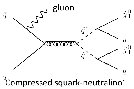
\includegraphics[width=\linewidth]{compressed}
    \caption{Event with initial state radiation~\cite{ExotPub}.}
    \label{fig:susy_compressed}
  \end{subfigure}
  \caption{Event topology of squark pair production resulting in a neutralinos
    with two jets final state with (\cref{fig:susy_compressed}) and without
    (\cref{fig:susy_standard}) initial state radiation.}
  \label{fig:motivation}
\end{figure}

\begin{figure}[!h]
  \centering
  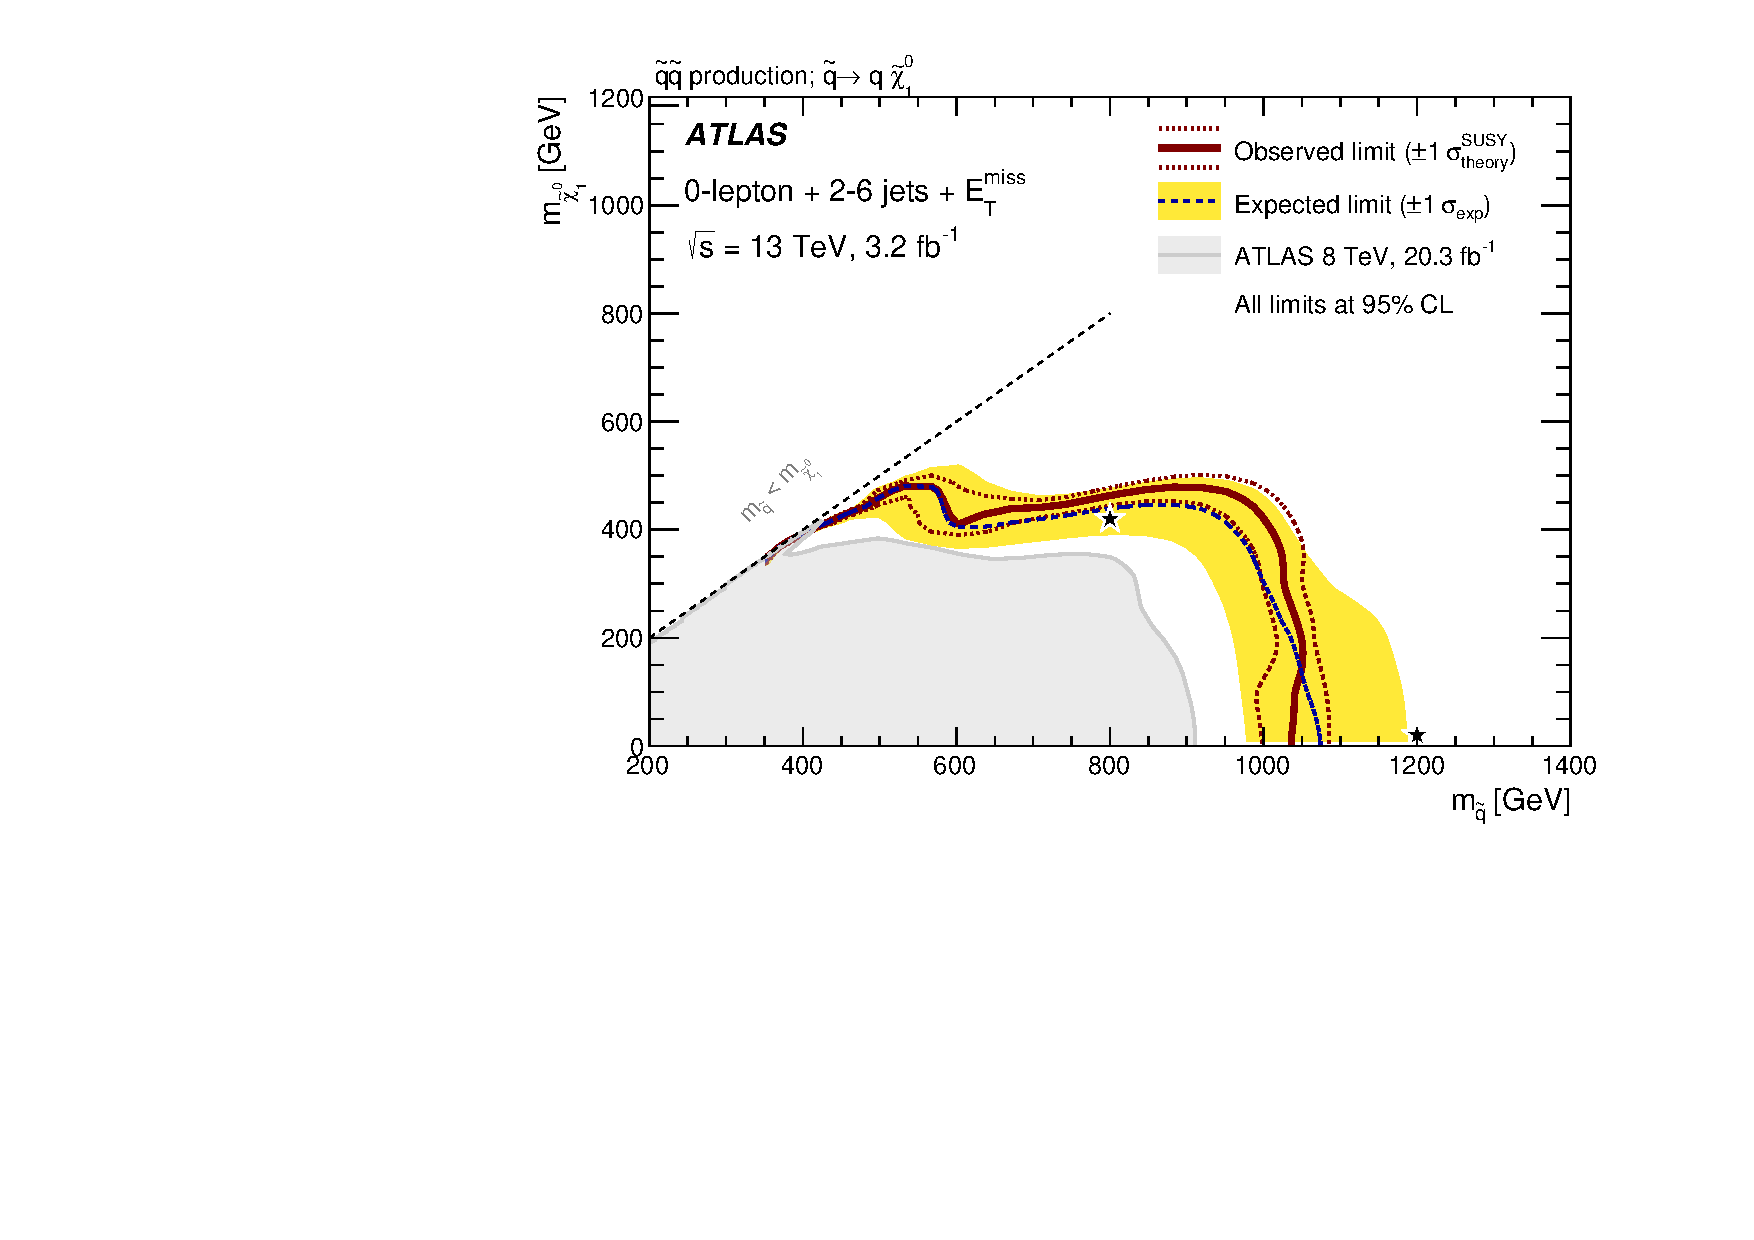
\includegraphics[width=.7\linewidth]{susy}
  \caption{Exclusion limits for direct production of squark
    pairs~\cite{SUSYPub}.}
  \label{fig:susy_exclusion}
\end{figure}
%%% Local Variables:
%%% mode: latex
%%% TeX-master: "../search_for_DM_LED_with_ATLAS"
%%% End:
